%% IMPORTANT: Once working, run latex 3 times to get listoffigures to work

%% Be sure to check spelling!

%% Put **your** name and the proper due date in place

%% Note put your own file names in the appendix
%% Copy the relevant code as many times as needed for all files

%% Note that the \epsfig command is currently commented out

\documentclass{article}
\usepackage{amsmath}    % load AMS-Math package
\usepackage{epsfig}     % allows PostScript files
\usepackage{listings}   % allows lstlisting environment
\usepackage{moreverb}   % allows listinginput environment
\usepackage{vmargin}    % allows better margins
\usepackage{multirow}   % allows multirow items in tabular
\usepackage{rotating}   % allows rotated pages
\setpapersize{USletter} % sets the paper size
\setmarginsrb{1in}{0.5in}{1in}{0.2in}{12pt}{11mm}{0pt}{11mm} %sets margins 
\begin{document}
\begin{center}
\rule{6.5in}{0.5mm}\\~\\
{\bf \large EGR 103L - Fall 2016}\\~\\
{\huge \bf Laboratory 8 - Intermediate Curve Fitting}\\~\\
CEMAL YAGCIOGLU\\
Lab Section 5D, Wednesday 11.45AM - 2.35PM\\
30 OCTOBER, 2016\\~\\
{\small I have adhered to the Duke Community Standard in completing
  this assignment.  I understand that a violation of the Standard can
  result in failure of this assignment, failure of this course, and/or
  suspension from Duke University.} 
\rule{6.5in}{0.5mm}\\
\end{center}
\tableofcontents
\listoffigures
\pagebreak
\renewcommand{\arraystretch}{1.5}

\section{Palm 6.10}
St value is equal to 57550.
% Complete tables
\begin{center}
\begin{tabular}{|c|c|} \hline
Order & Equation ($d=f(v)$)\\ \hline
1 & $(5.6857e+00) + (-8.5857e+01)x$ \\ \hline
2 & $(5.0893e-02) + (1.1054e+00)x   (2.3571e+00)x^2$ \\ \hline
3 & $(1.3889e-04) + (3.2143e-02)x + (1.8790e+00)x^2 + (-7.1429e+00)x^3$ \\ \hline
\end{tabular}
\end{center}

\begin{center}
\begin{tabular}{|c|c|c|c|c|c|c|c|} \hline
Order & $S_r$ & $r^2$ & $d(65)$ (ft) &
$d(100)$ (ft)\\ \hline
1 & 9.7714e+02 & 9.8302e-01 & 2.8371e+02 & 4.8271e+02 \\ \hline
2 & 1.0179e+01 & 9.9982e-01 & 2.8923e+02 & 6.2182e+02 \\ \hline
3 & 8.9286e+00 & 9.9984e-01 & 2.8894e+02 & 6.4107e+02 \\ \hline
\end{tabular}
\end{center}

Although r squared value increases with higher number of terms, 2nd degree polynomial and 3rd degree polynomial are both good representations of the given data. The increasing r squared value when passing from second degree to third degree is due to side effect of mathematics and does not add a scientifically significant term.

\section{Palm 6.16}
% give model with coefficients
Model is : $y=5.75ln(x)+9.91$. Thus a1=5.75 and a2=9.91.
% show statistical information
St, Sr and r2 values are respectively 160, 0.4145, 0.997.
% calculate and display estimates
Estimates for x=2.5 and x=11 are respectively 15.2, 23.7.
\section{Chapra 15.12}
% give model with coefficients
Model is :  $y= 3.7450e-01 + (9.8644e-01)x + (8.4564e-01)x^{-1}$
% show statistical information
St, Sr and r2 values are respectively 6.9480e+00, 2.7651e-03, 9.9960e-01.
% calculate and display estimates
Estimates for x=1.5 and x=4.5 are respectively 2.4179e+00, 5.0014e+00.

\section{Chapra 14.12}
% give model with coefficients
Model is : $W=(4.1489e-01)*A^{3.7991e-01}$
% show statistical information
St, Sr and r2 values are respectively 7.0102e-03, 2.0240e-04, 9.7113e-01.
% calculate and display estimate
Estimate for W=95 is 2.3404e+00(meters squared).

\section{Chapra 14.14}
% give model with coefficients
Model is : $k=((1.0345e+01)*c^2)/(2.0897e+00+c^2)$
% show statistical information
St, St and r2 values are respectively 4.4527e-01, 1.9178e-04, 9.9957e-01.
\section{Chapra 15.7}

% give model with coefficients
Model is : $ OC=(-1.0493e-01)c + (-4.3704e-05)T^3 + (5.7444e-03)T^2 + (-3.3642e-01)T + 1.4027e+01 $
% show statistical information
St, Sr and r2 values are respectively 1.0400e+02, 1.2784e+00, 9.8771e-01.
% calculate and display estimate
Estimate for T=12 and c=15 is 9.1678e+00.
% discuss model
For this model, r2 value is high, indicating a good mathematical fit. Also relative error for given point is small, which tells that exptrapolation can be accurately used meaning its a good mathematical fit.
% calculate relative error
Relative error is equal to 8.5605e-03.

\section{Chapra 15.10}
% give model with coefficients
Model is : $p(t)= (4.1375e+00)e^{-1.5t} +  (2.8959e+00)e^{-0.3t} + (1.5349e+00)e^{-0.05t}$
% show statistical information
St, Sr and r2 values are respectively 2.0409e+01, 8.0348e-02, 9.9606e-01.
% discuss model
In this model, r2 value is high indicating a mathetically fit model. Also, as expected for decay, all graphs show decrease. Thus its a mathematically good model. 
\section{Chapra 15.10 Alternate}
% give model with coefficients
Model is : $p(t)= (5.6328e+00)e^{-1.5t} +  (-4.4272e+00)e^{-0.3t} + (7.8906e+00)e^{-0.2t}$  
% show statistical information
St, Sr and r2 values are respectively 2.0409e+01, 7.9611e-02, 9.9610e-01.
% discuss model, and compare mathematically and scientifically with original
This model has a higher r2 value, however Decay B starts from a negative value which is not scientificially accurate as a population cannot be negative. Thus, it is not a scientifically accurate model.

\section{Chapra 14.11 (Linearized)}
St is equal to 5.4240e+04.
% Complete table:
\begin{center}
\begin{tabular}{|c|c|c|c|c|}\hline 
Fit & Equation & $S_r$ & $r^2$ & Tiger M. (watts) \\\hline 
Exp.    & $M=(5.3509e+00)~e^{((1.1138e-02)~m)}$    & 4.2972e+04 &  2.0773e-01 &  4.9640e+01  \\\hline
Power   & $M=(3.3893e+00)~m^{(7.2656e-01)}$         & 1.1874e+02 &  9.9781e-01 &  1.5920e+02  \\\hline
Sat.~G. & $M=(2.1011e+01 )\frac{m}{(3.4857e+00)+m}$ & 6.6866e+04 &  -2.3279e-01 &   2.0651e+01  \\\hline
\end{tabular}
\end{center}

\section{Chapra 14.11 (Nonlinear Regression)}
% Present St and fill out the table, then answer discussion questions
St is equal to 5.4240e+04.
\begin{center}
\begin{tabular}{|c|c|c|c|c|}\hline 
Fit & Equation & $S_r$ & $r^2$ & Tiger M. (watts) \\\hline 
Exp.    & $M=(2.6088e+01)~e^{((5.8543e-03)~m)}$    & 3.7901e+03 & 9.3012e-01 & 8.4128e+01 \\\hline
Power   & $M=(3.5436e+00)~m^{(7.2345e-01)}$         & 6.2197e+01 & 9.9885e-01 & 1.6373e+02  \\\hline 
Sat.~G. & $M=(5.5198e+02)\frac{m}{(4.1748e+02)+m}$ & 2.7645e+01 & 9.9949e-01 & 1.7878e+02  \\\hline 
\end{tabular}
\end{center}

 
\pagebreak
\appendix
\section{Codes and Output}
% Put the name of your file in the subsection name 
% and the listinginput input
% Be sure to include the community standard in codes!
% Add \pagebreaks if they make sense
% Make as many copies as you need

\subsection{ONE.m}
\listinginput[1]{1}{ONE.m}
\pagebreak


\subsection{TWO.m}
\listinginput[1]{1}{TWO.m}
\pagebreak


\subsection{THREE.m}
\listinginput[1]{1}{THREE.m}
\pagebreak


\subsection{FOUR.m}
\listinginput[1]{1}{FOUR.m}
\pagebreak


\subsection{FIVE.m}
\listinginput[1]{1}{FIVE.m}
\pagebreak



\subsection{SIX.m}
\listinginput[1]{1}{SIX.m}
\pagebreak


\subsection{SEVEN.m}
\listinginput[1]{1}{SEVEN.m}
\pagebreak

\subsection{EIGHT.m}
\listinginput[1]{1}{EIGHT.m}
\pagebreak

\subsection{NINE.m}
\listinginput[1]{1}{NINE.m}
\pagebreak

\subsection{TEN.m}
\listinginput[1]{1}{TEN.m}
\pagebreak






\section{Figures}
% Make as many as needed; change sizes if it makes sense to do so
\begin{figure}[h!]
\begin{center}
%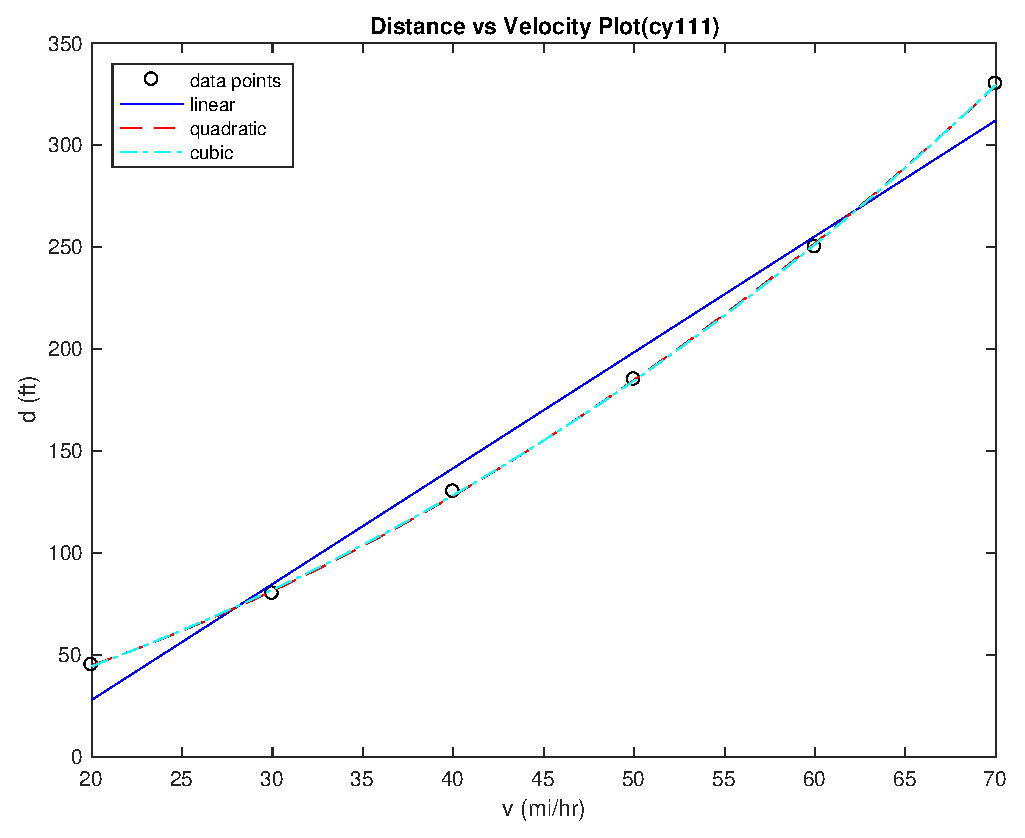
\epsfig{file=DistanceVelocityPlot.eps, width=2.7in}
\caption{Distance Velocity Plot}
\end{center}
\end{figure}



% Make as many as needed; change sizes if it makes sense to do so
\begin{figure}[h!]
\begin{center}
%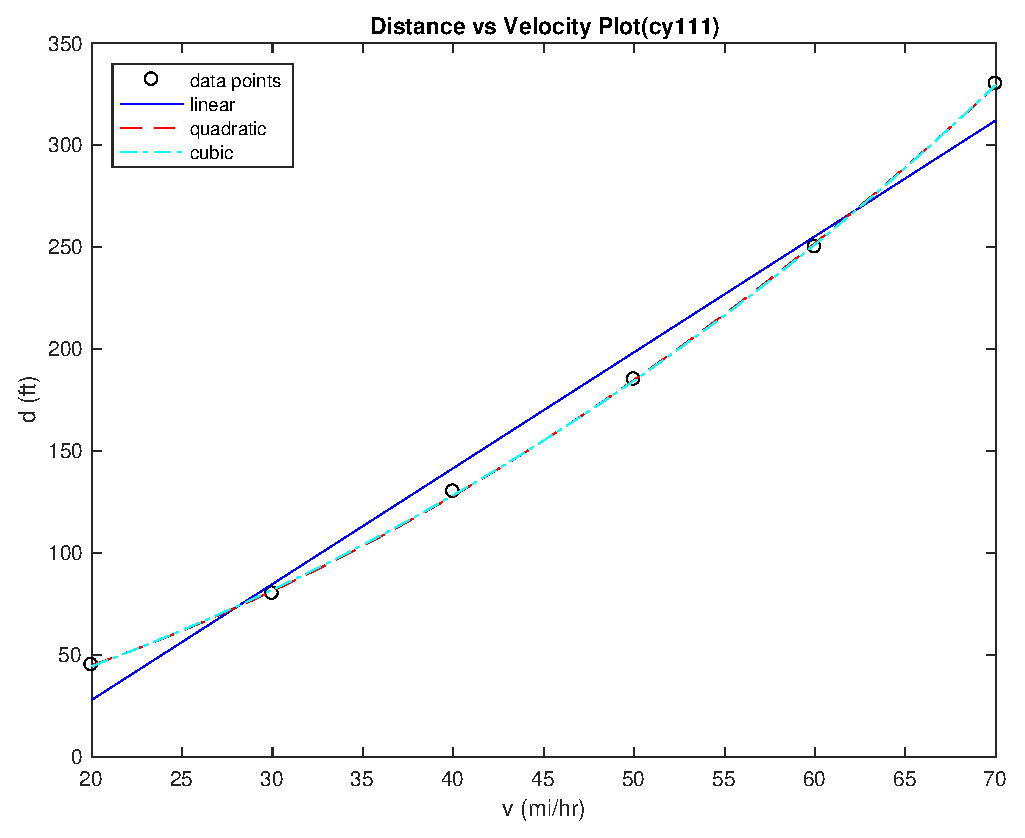
\epsfig{file=DistanceVelocityPlot.eps, width=2.7in}
\caption{Distance Velocity Plot}
\end{center}
\end{figure}

% Make as many as needed; change sizes if it makes sense to do so
\begin{figure}[h!]
\begin{center}
%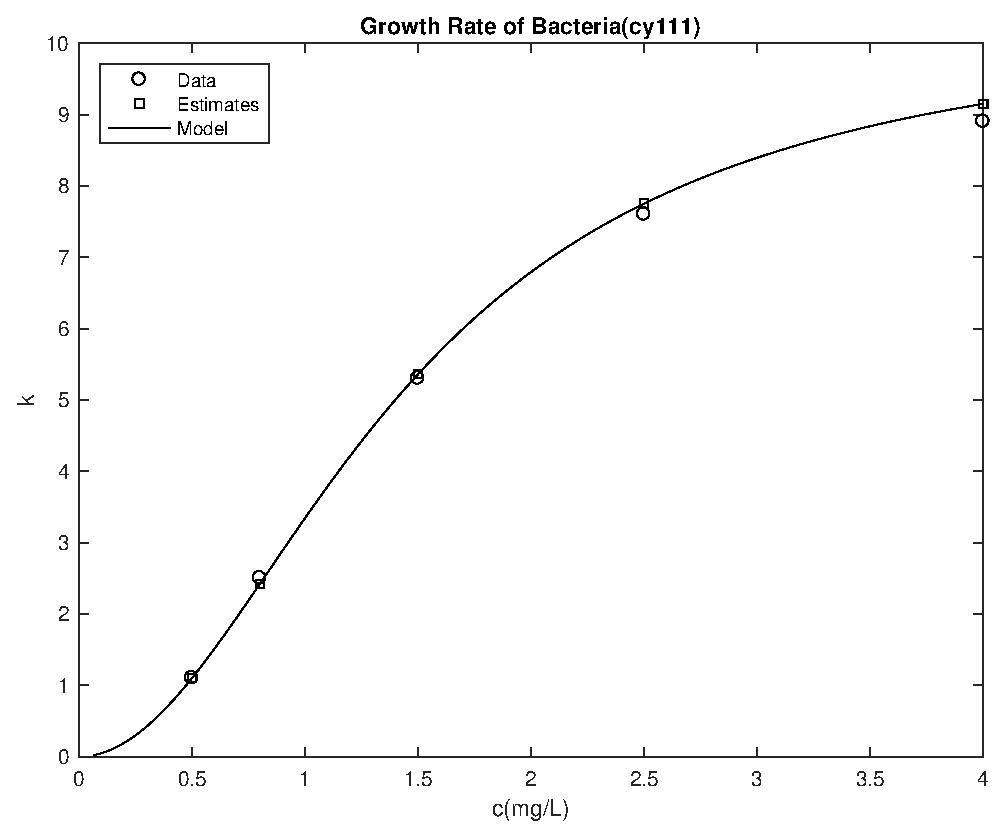
\epsfig{file=BacteriaPlot.eps, width=2.7in}
\caption{Bacteria Plot}
\end{center}
\end{figure}

% Make as many as needed; change sizes if it makes sense to do so
\begin{figure}[h!]
\begin{center}
%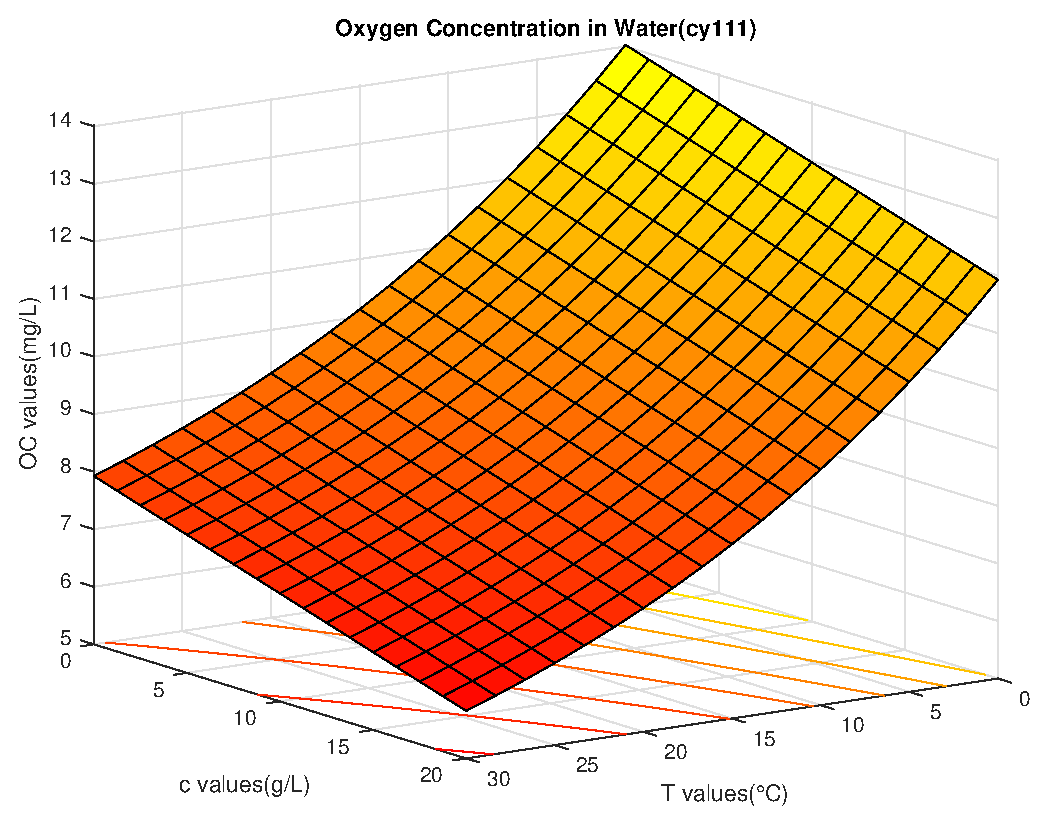
\epsfig{file=OxygenConcentration, width=2.7in}
\caption{Oxygen Concentration Surface}
\end{center}
\end{figure}

% Make as many as needed; change sizes if it makes sense to do so
\begin{figure}[h!]
\begin{center}
%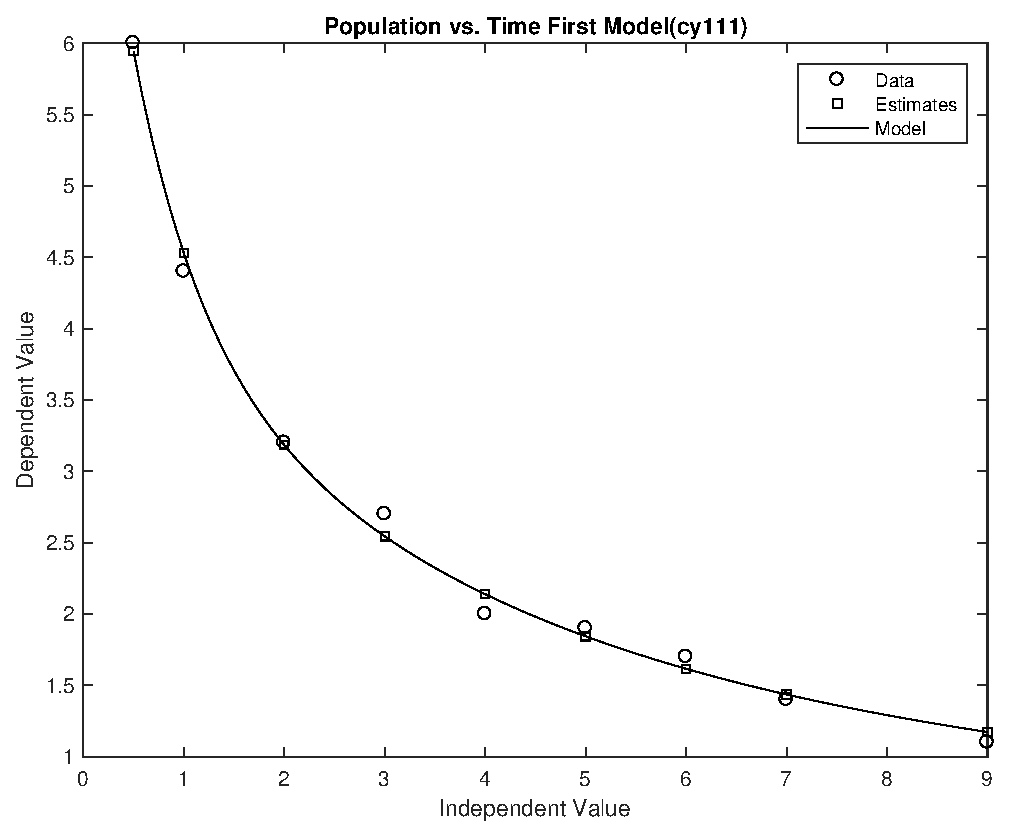
\epsfig{file=Decay11.eps, width=2.7in}
\caption{Population vs Time First Model}
\end{center}
\end{figure}


\begin{figure}[h!]
\begin{center}
%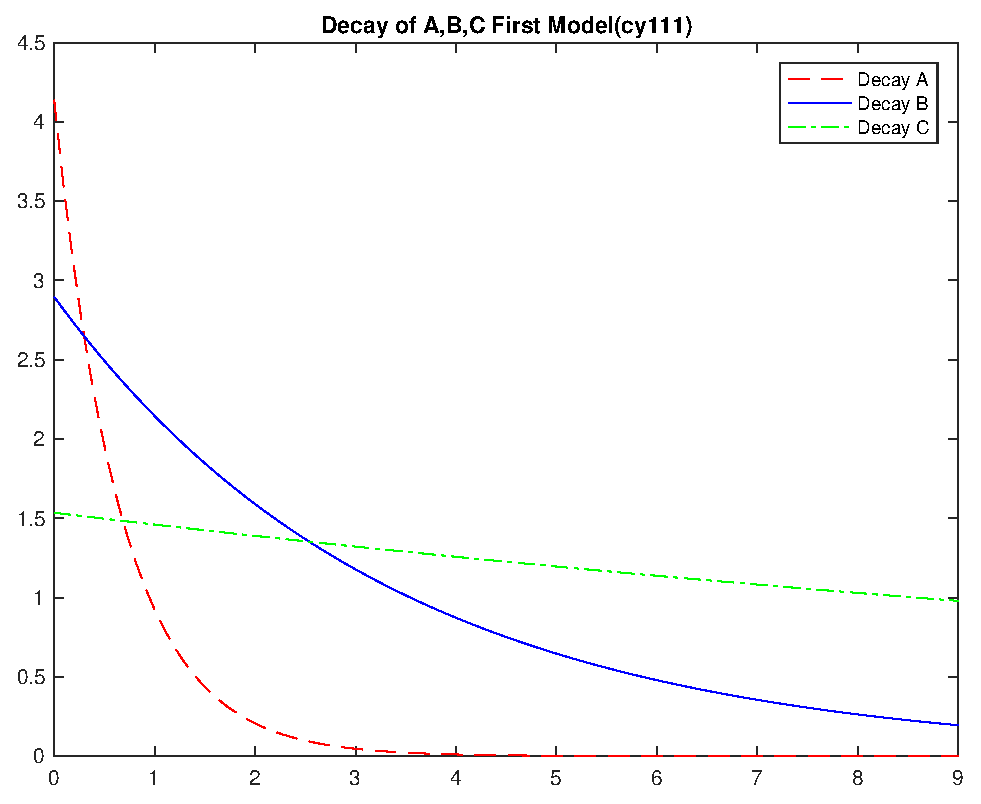
\epsfig{file=Decay12.eps, width=2.7in}
\caption{Decay of A,B,C First Model}
\end{center}
\end{figure}


\begin{figure}[h!]
\begin{center}
%\epsfig{file=Decay21.eps, width=2.7in}
\caption{Population vs Time Second Model}
\end{center}
\end{figure}



\begin{figure}[h!]
\begin{center}
%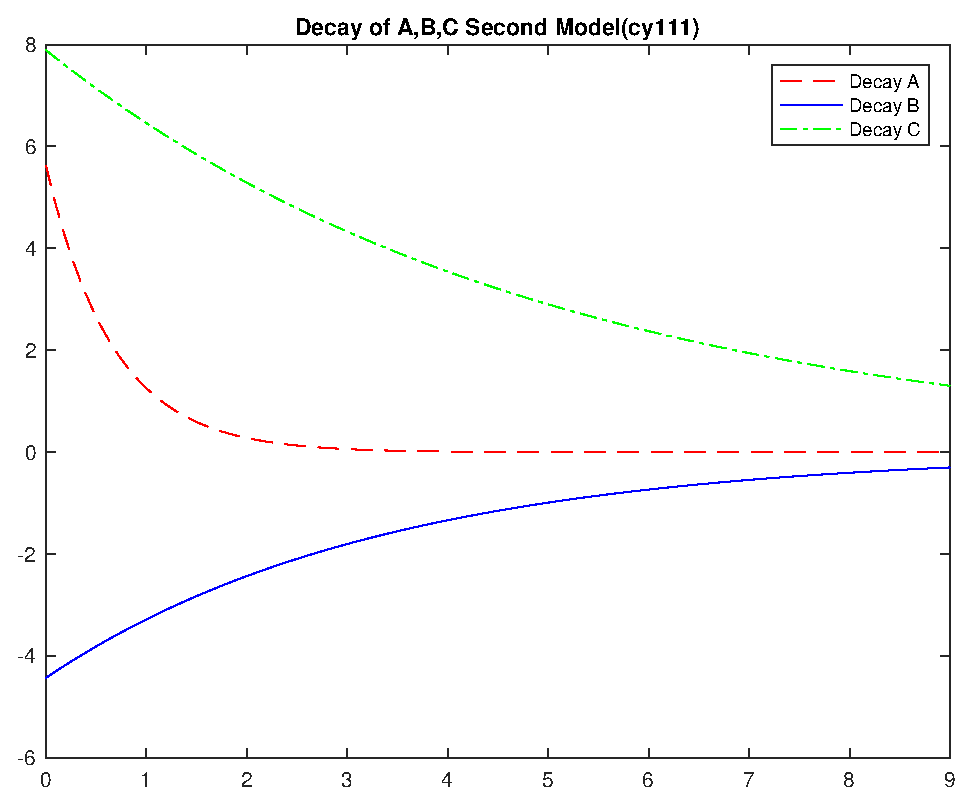
\epsfig{file=Decay22.eps, width=2.7in}
\caption{Decay of A,B,C Second Model}
\end{center}
\end{figure}




% Here's the way to organize the last sets of plots:
\begin{sidewaysfigure}[h!]
\begin{center}
\begin{tabular}{ccc}
%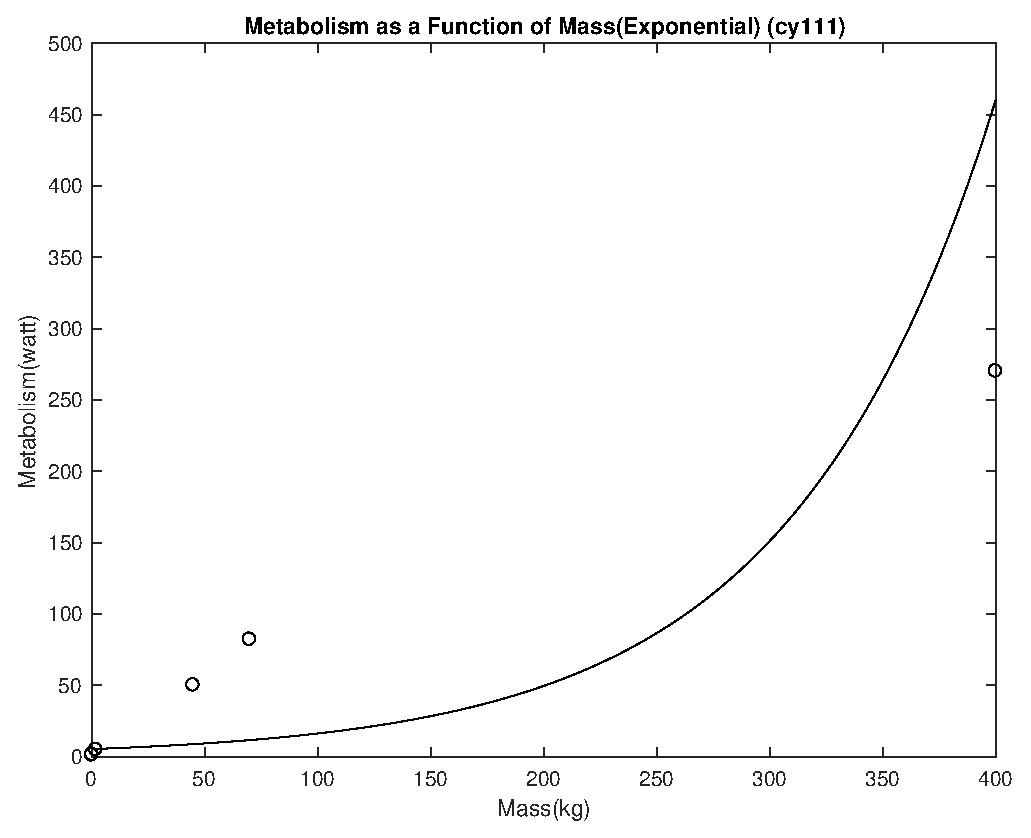
\epsfig{file=./M11.eps, width=2.5in, height=2.5in} & 
%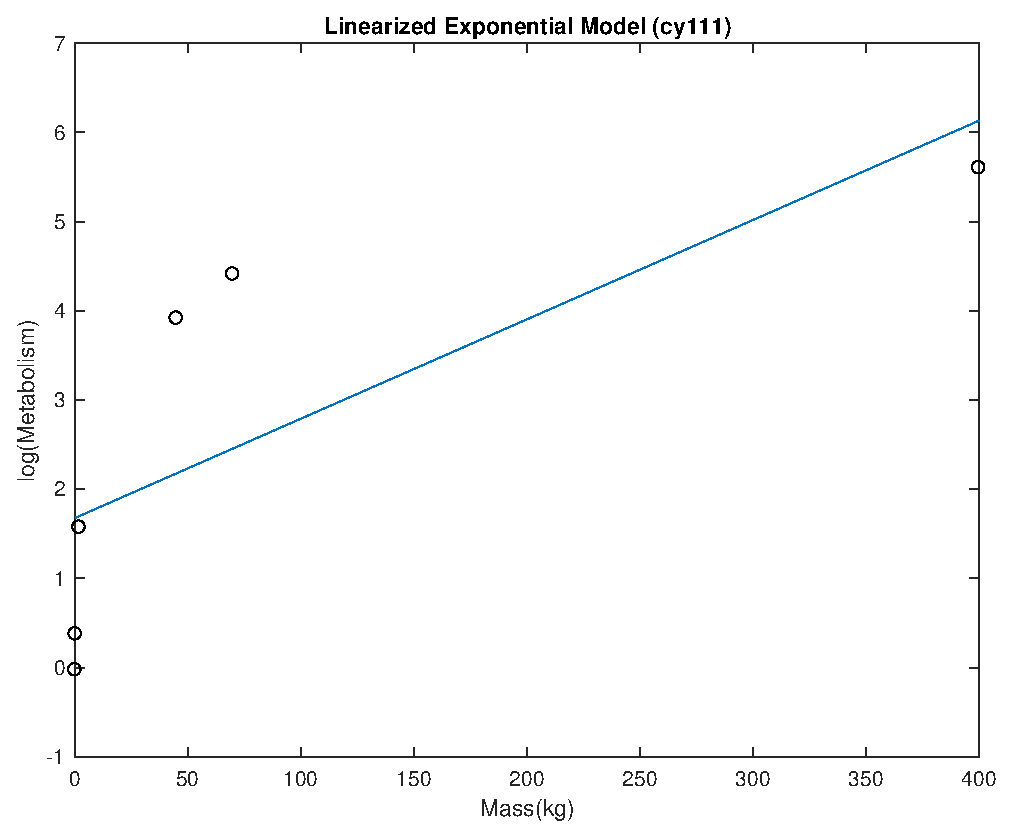
\epsfig{file=./M12.eps, width=2.5in, height=2.5in} &
%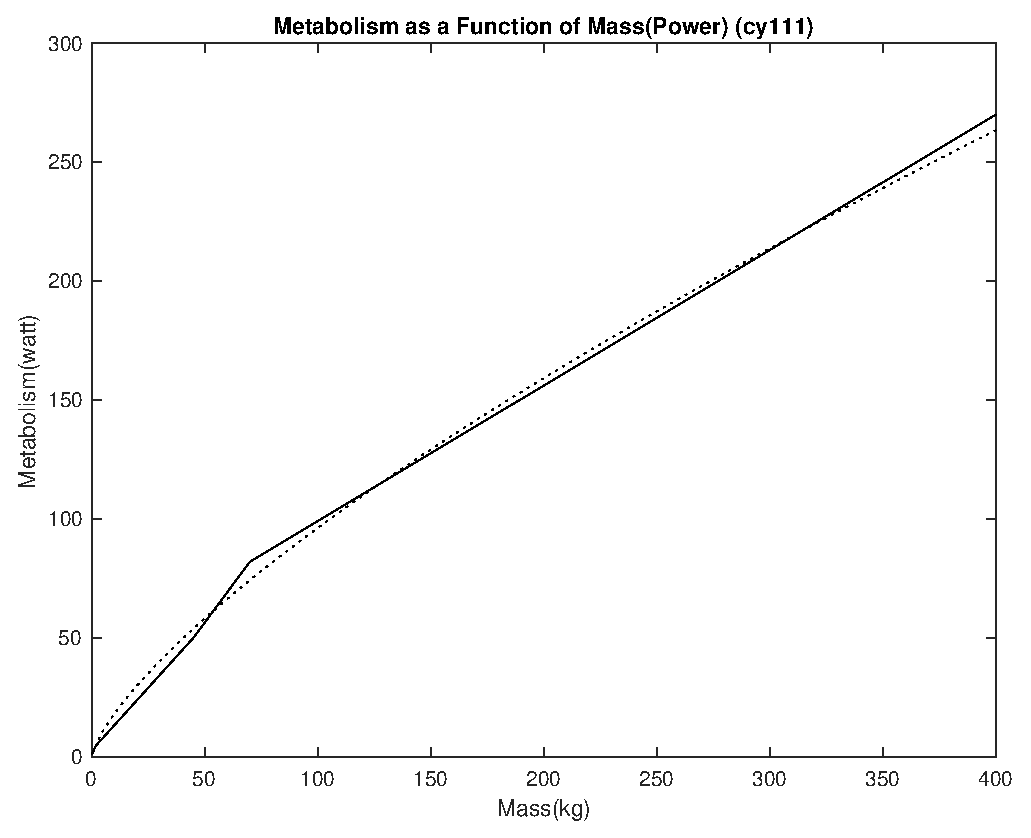
\epsfig{file=./M13.eps, width=2.5in, height=2.5in} \\
%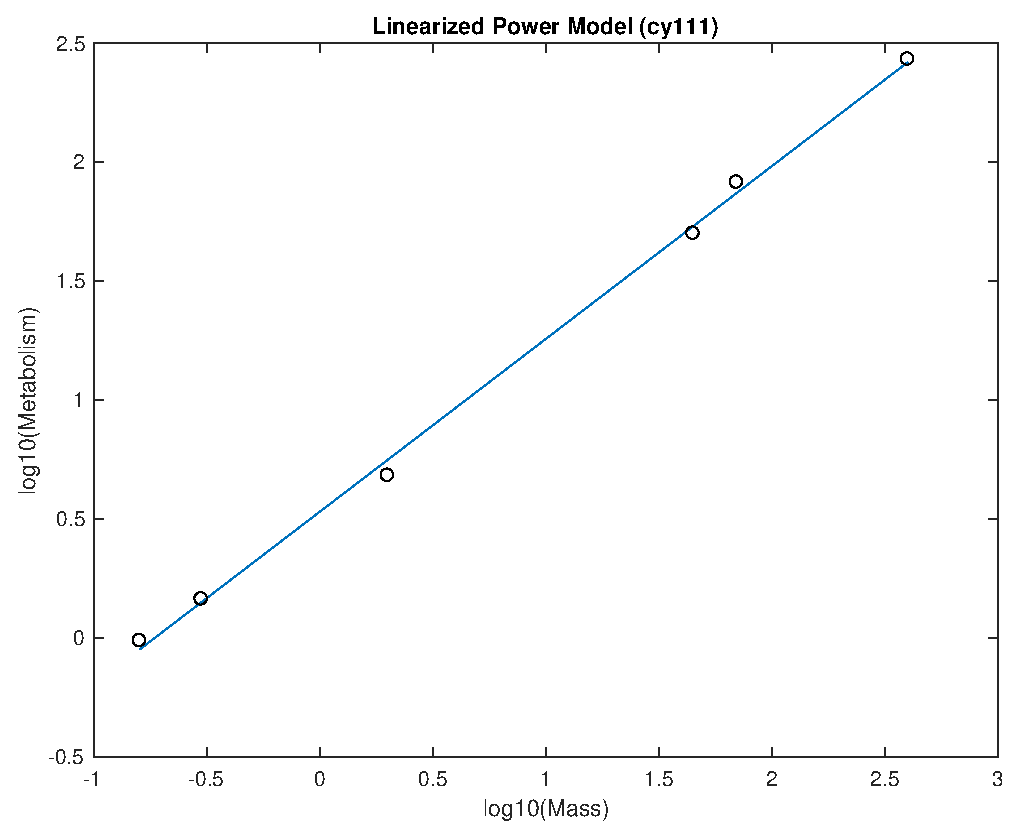
\epsfig{file=./M14.eps, width=2.5in, height=2.5in} & 
%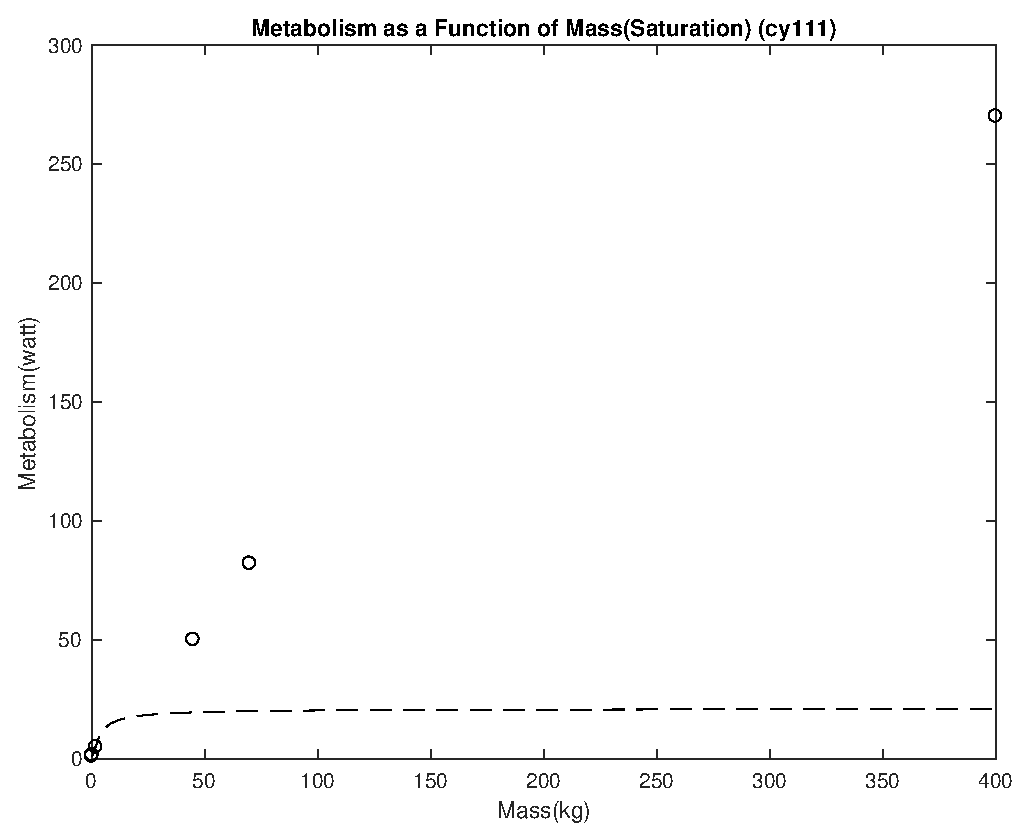
\epsfig{file=./M15.eps, width=2.5in, height=2.5in} & 
%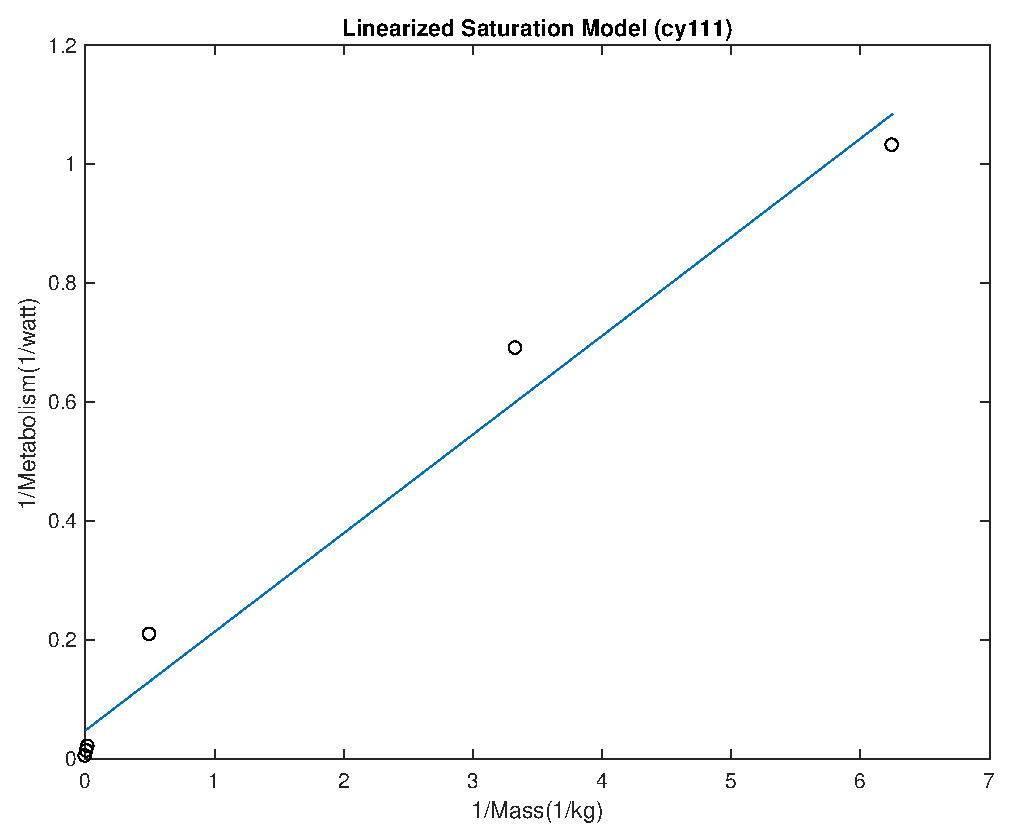
\epsfig{file=./M16.eps, width=2.5in, height=2.5in}
\end{tabular}
\end{center}
\caption{Untransformed and Transformed Plots for Linearized Metabolism Models}
\end{sidewaysfigure}

\begin{sidewaysfigure}[h!]
\begin{center}
\begin{tabular}{ccc}
%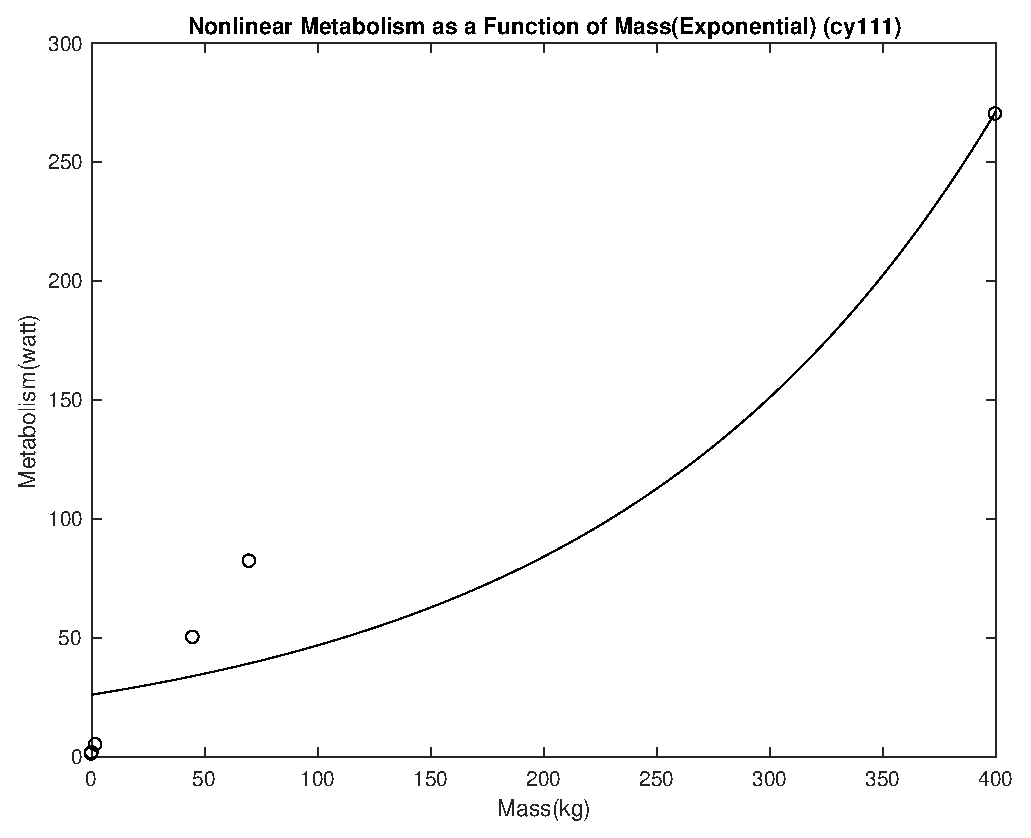
\epsfig{file=./M21.eps, width=2.5in, height=2.5in} & 
%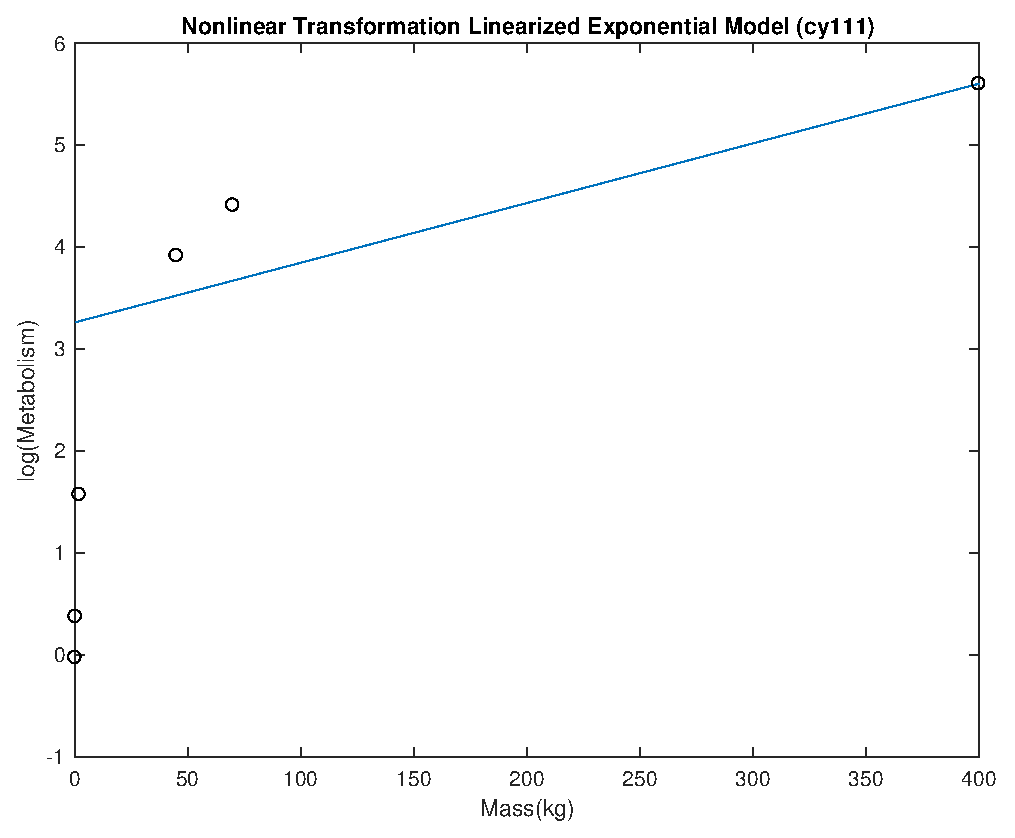
\epsfig{file=./M22.eps, width=2.5in, height=2.5in} &
%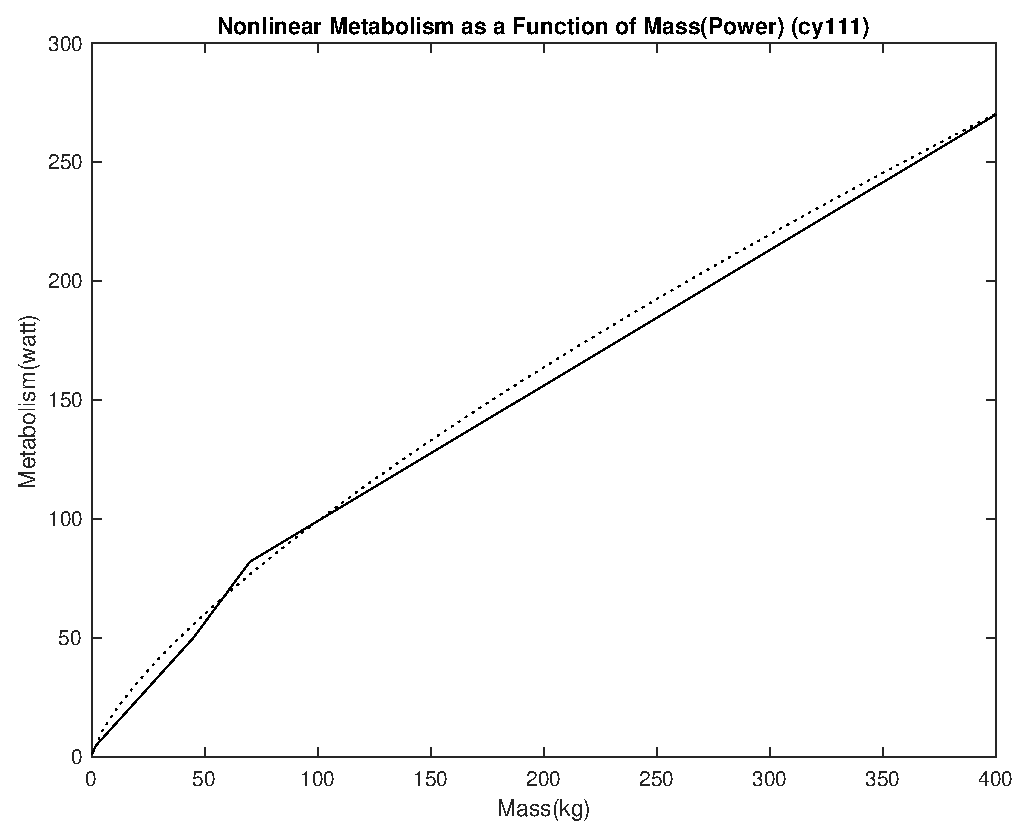
\epsfig{file=./M23.eps, width=2.5in, height=2.5in} \\
%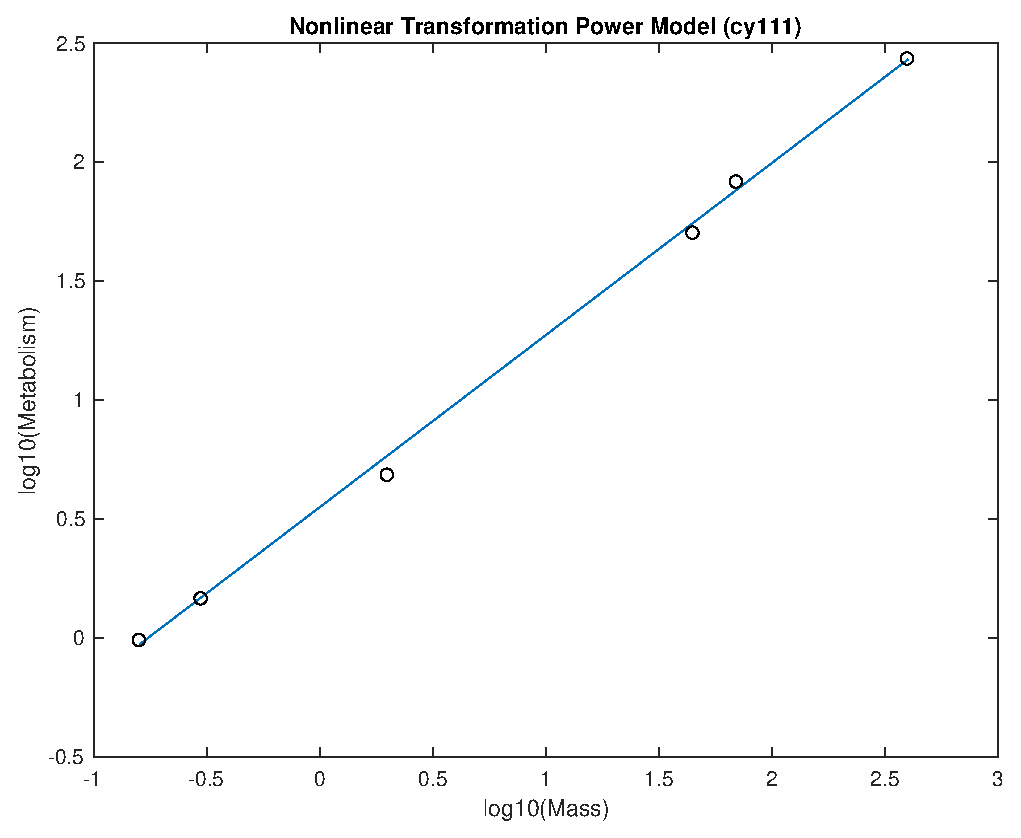
\epsfig{file=./M24.eps, width=2.5in, height=2.5in} & 
%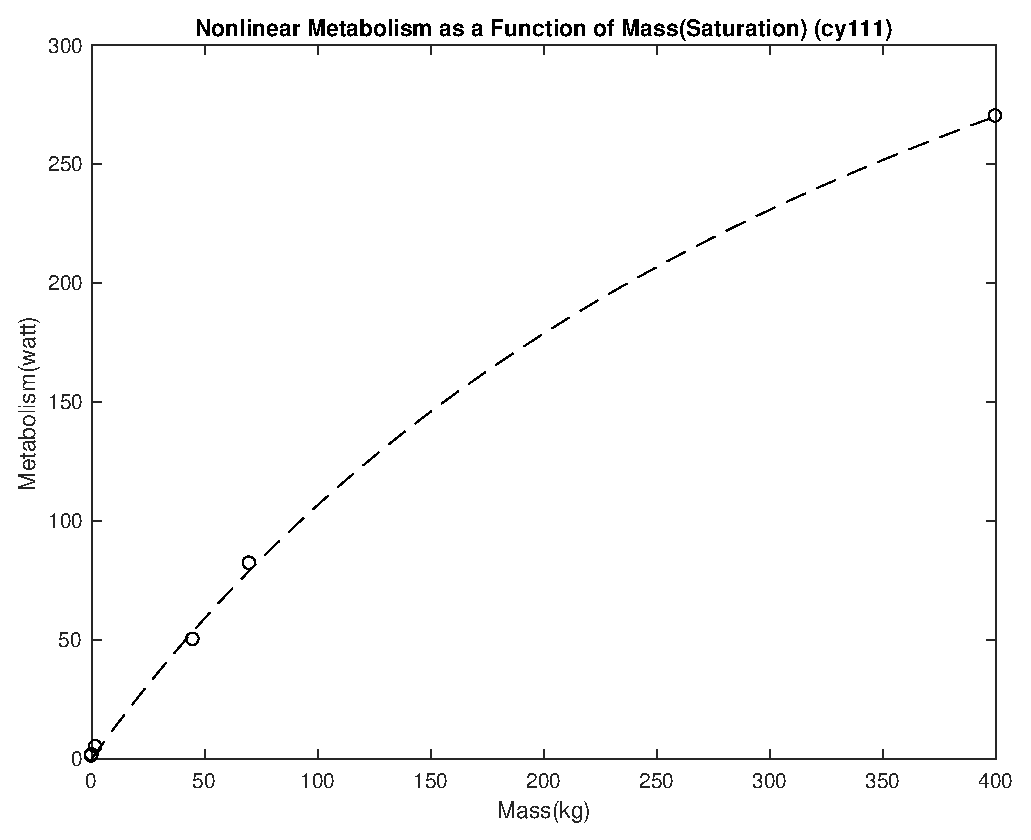
\epsfig{file=./M25.eps, width=2.5in, height=2.5in} & 
%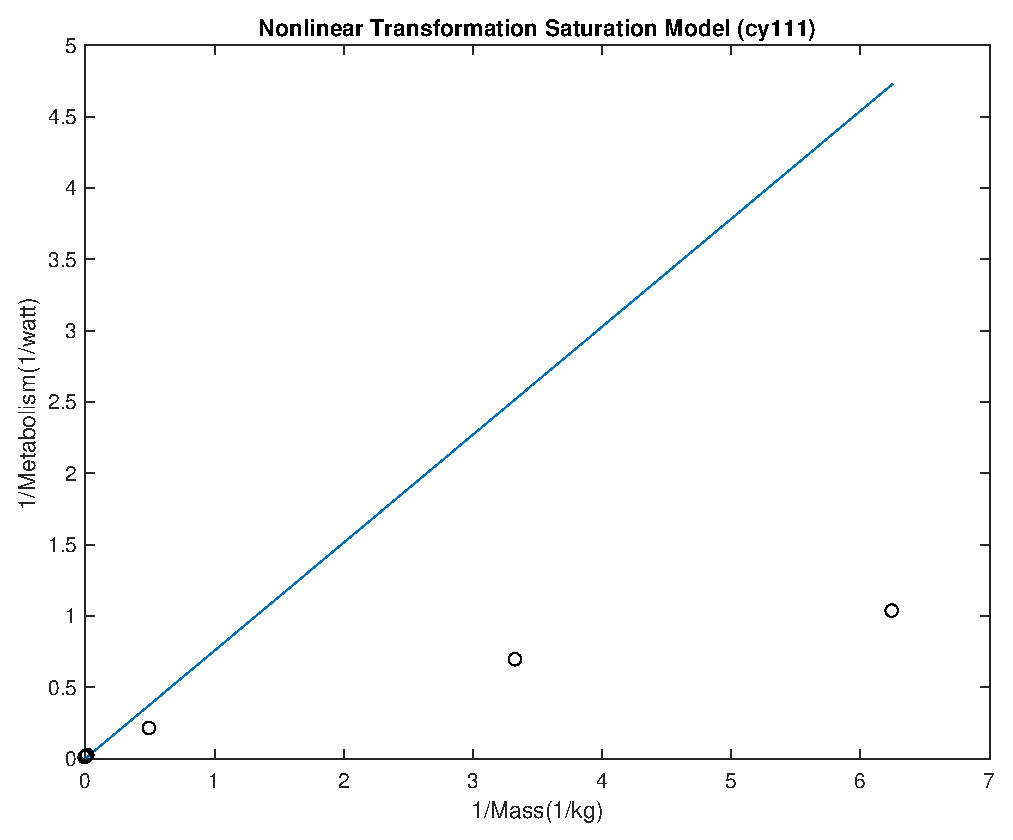
\epsfig{file=./M26.eps, width=2.5in, height=2.5in}
\end{tabular}
\end{center}
\caption{Untransformed and Transformed Plots for Unlinearized Metabolism Models}
\end{sidewaysfigure}
\clearpage


\end{document}

% LocalWords:  EGR 103L Chapra untransformed Linearized
